\chapter{Controleren van consistentie}\label{sec:consistentie}
In dit hoofdstuk treden we meer in detail over hoe we de consistentie van een diagram willen controleren. Daarvoor willen we een specifieke vorm van logische theorie automatisch laten genereren. In deze theorie\"en staan \textbf{objecten} centraal. Deze objecten zijn instanties van een klasse die voorkomt in het beschouwde diagram, hebben exact de attributen en operaties van die klasse en maken deel uit van exact die relaties die het diagram voorschrijft voor die klasse. Aan de hand van volgend voorbeeld zullen we illustreren welke regels we gebruiken om zulk een theorie op te bouwen:

\begin{figure}[H]
	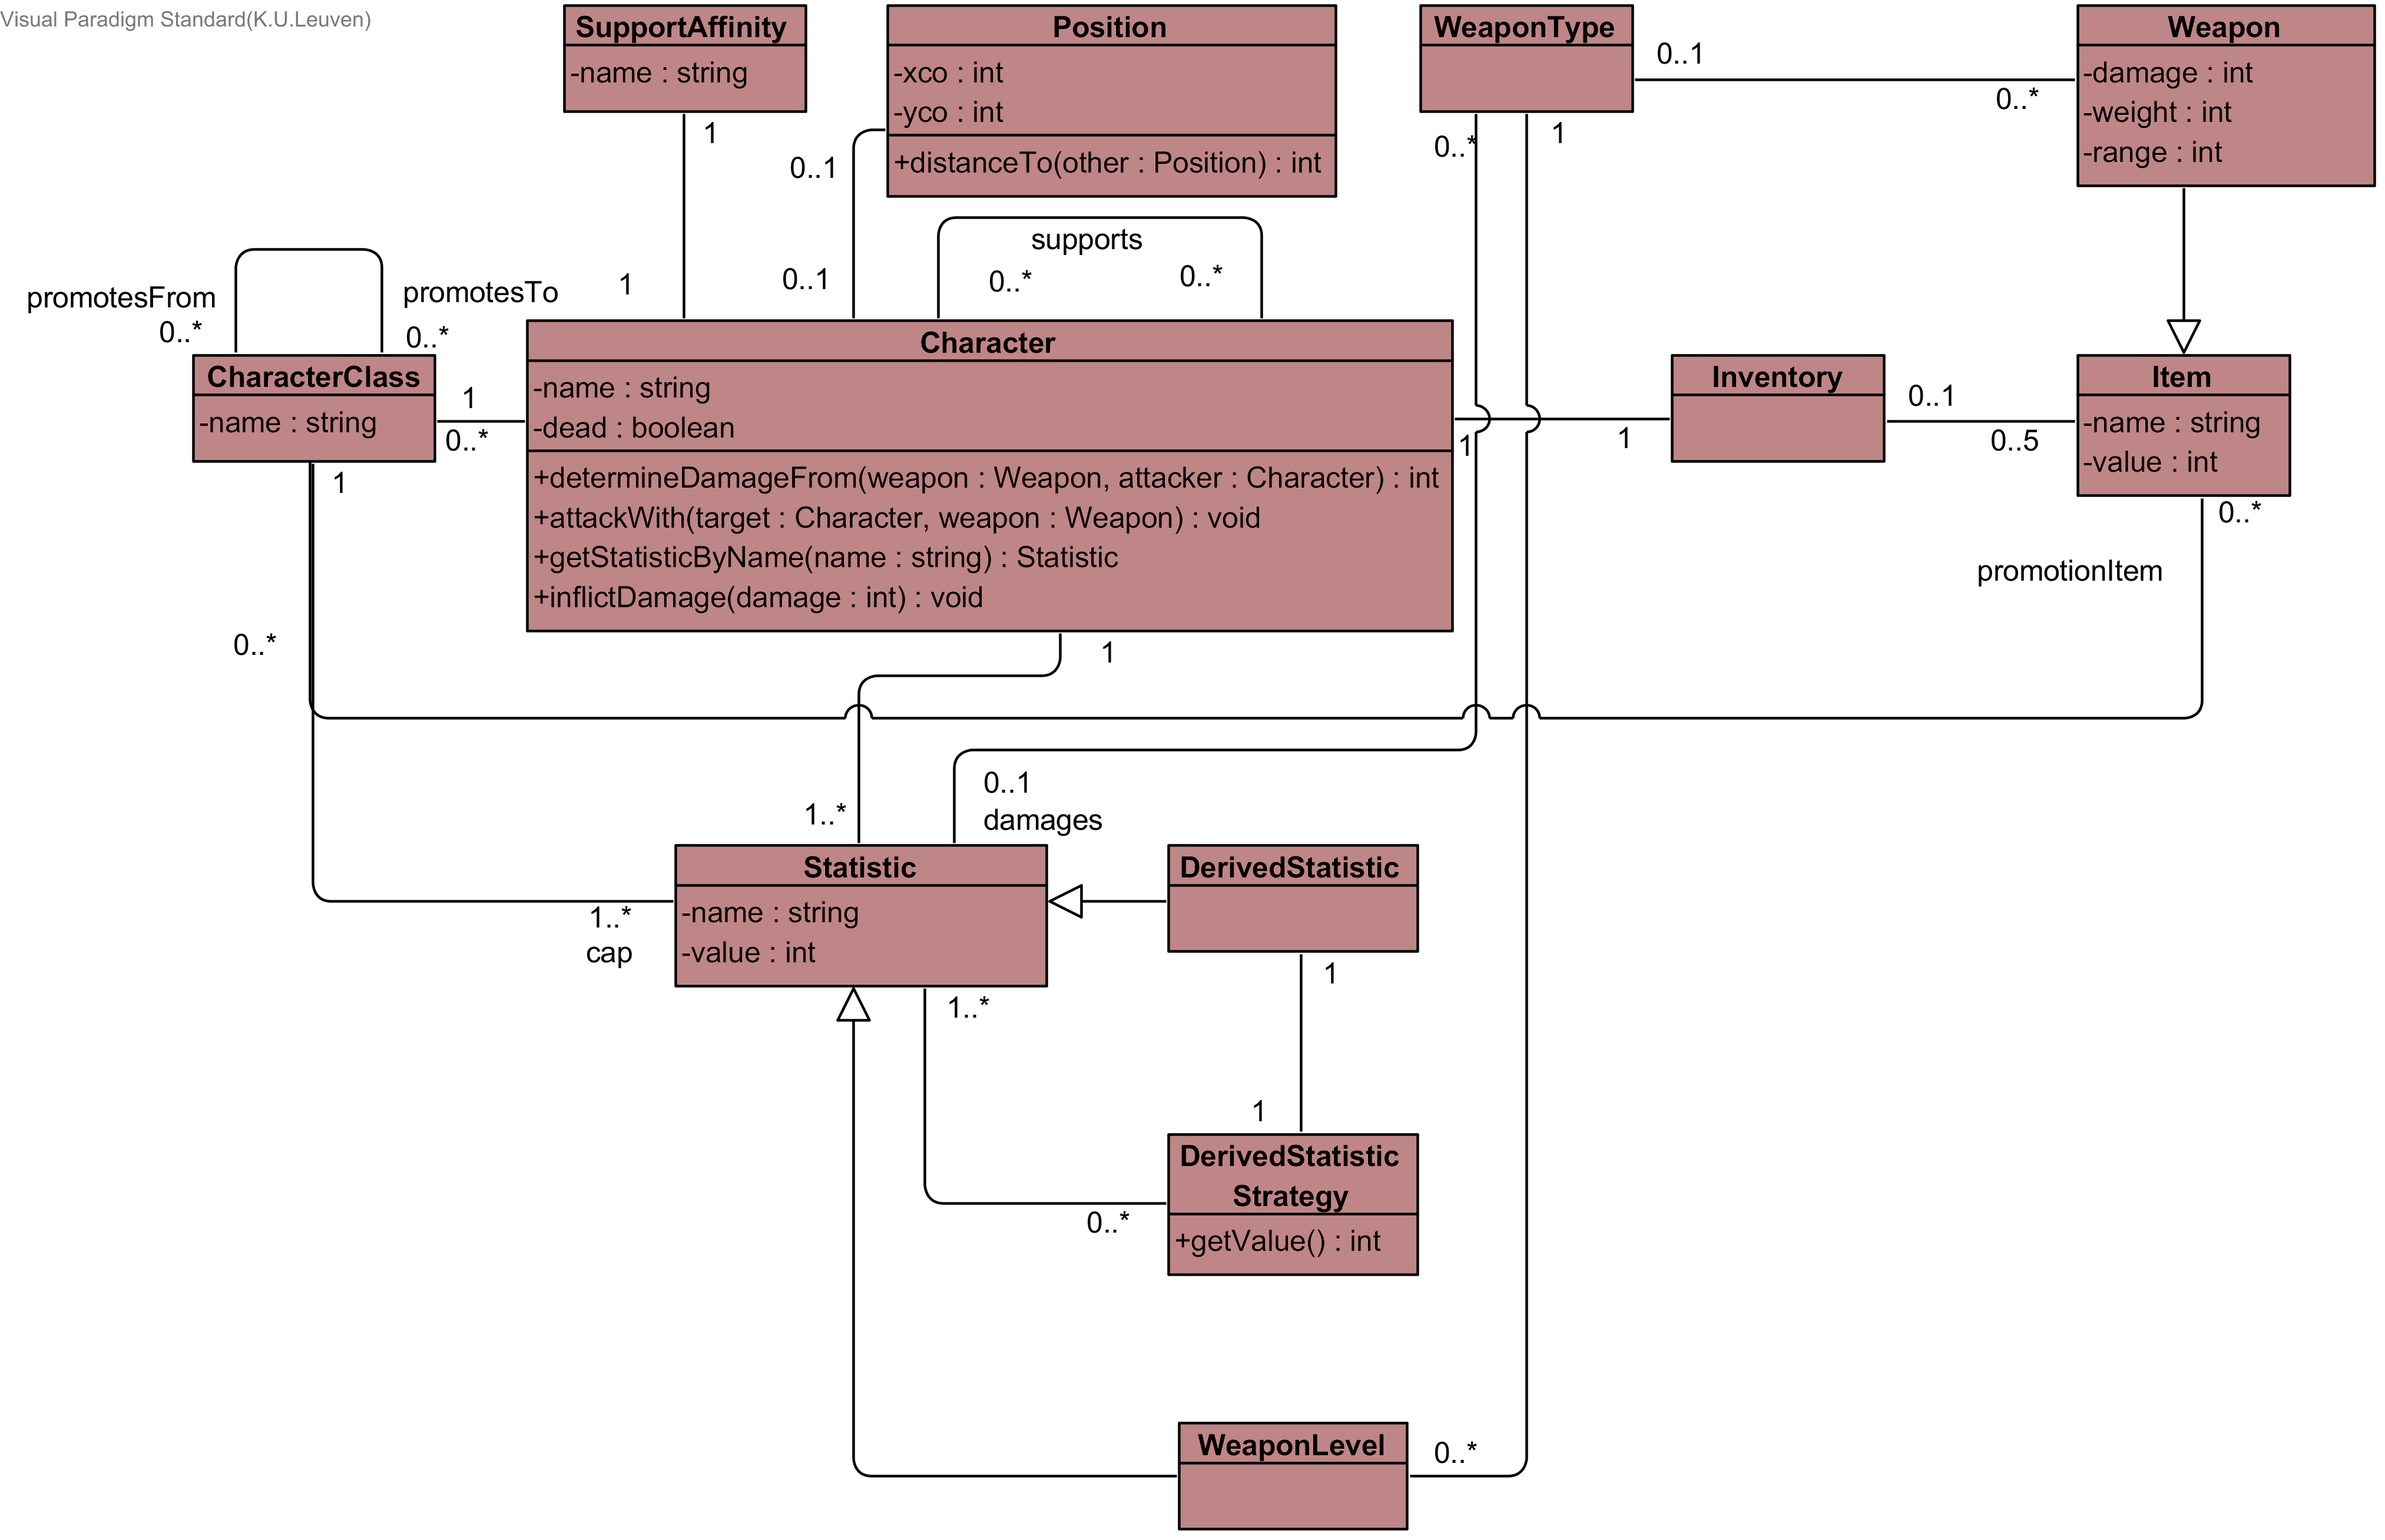
\includegraphics[width=0.95\textwidth]{chap-consistentie/diagram-voorbeeld.png}
	\caption{Leidend voorbeeld van een klassediagram}
	\label{fig:diagram-voorbeeld}
\end{figure}

Meer bepaald willen we uitdrukken welke \textbf{klasses} er bestaan in het diagram waarvan een object een instantie kan zijn, welke \textbf{attributen} en \textbf{operaties} elke klasse bevat, welke \textbf{associaties} er bestaan tussen de verscheidene klasses en welke \textbf{klassehi\"erarchie\"en} er bestaan.

\subsection{Logisch type \textit{Object}}
Zoals gezegd staan in deze theori\"en objecten centraal, dus is het vanzelfsprekend om een logisch type \textit{Object} te voorzien. Dit logisch type bevat dus softwareobjecten.

\subsection{Logisch type \textit{ClassObject} en predicaat \textit{StaticClass$\backslash2$}}
Dit logisch type bevat exact de klasses die worden weergegeven in het diagram --- niet meer en niet minder. \textit{Character}, \textit{Inventory}, \textit{Item} enz. zijn dus \textit{ClassObject}s.
We drukken uit dat een \textit{Object} een instantie is van een bepaald \textit{ClassObject} door middel van het predicaat \textit{StaticClass$\backslash2$}. \textit{StaticClass(o1,Character)} zegt dus uit dat het object \textit{o1} een instantie is van klasse \textit{Character}.

\subsection{Voorstellen van attributen}
Voor elk attribuut voegen we een binair predicaat toe waarvan de naam beantwoordt aan het patroon: \textit{Klassenaamattribuutnaam}. Voor klasse \textit{Character} en attribuut \textit{name} resulteert dit dus in het predicaat \textit{Charactername$\backslash2$}. Het eerste argument van dit predicaat is een \textit{Object}. Het type van het tweede argument hangt af van wat er in het diagram staat: Als het een primitief type is zoals \textit{string} of \textit{int}, zal dat ook het type zijn van het tweede predicaat; in het andere geval is het type van het tweede argument ook \textit{Object}.
De signatuur van \textit{Charactername$\backslash2$} is daarom \textit{Charactername(Object, string)}.
Voor elk attribuut worden ook een aantal andere regels afgeleid:

\begin{itemize}
	\item Als het tweede argument van het attribuutpredicaat \textit{Object} is, wordt er een regel toegevoegd van de vorm:
	
	\begin{align*}
	\forall{o1}[Object]\forall{o2}[Object](Klassenaamattribuutnaam(o1,o2) \Rightarrow \\ StaticClass(classObj,o1) \land StaticClass(attrClassObj,o2))
	\end{align*}
	
	waarbij \textit{classObj} het logisch object van type \textit{ClassObject} dat het attribuut bevat en \textit{attrClassObj} het logisch object van type \textit{ClassObject} dat dient als mogelijke waarde van dit attribuut. Deze regel verzekert dat de attribuuthouder en de attribuutwaarde van de juiste klasse zijn. In dit diagram komt dit geval nergens voor en wordt deze regel dus niet toegepast.
	
	\item Als het tweede argument van het attribuutpredicaat van een primitief type is, wordt een regel toegevoegd van de vorm:
	
	\begin{align*}
	\forall{o}[Object]\forall{x}[primitiveType](Klassenaamattribuutnaam(o,x) \Rightarrow \\ StaticClass(classObj,o))
	\end{align*}
	
	waarbij primitiveType het type van de attribuutwaarde. De signatuur van het predicaat verzekert dat de attribuutwaarde van het juiste type is, dus moet dit niet explicit worden neergeschreven. Deze regel zorgt ervoor dat de volgende zin wordt toegevoegd aan de theorie:
	
	\begin{align*}
	\forall{o}[Object]\forall{x}[primitiveType](Charactername(o,x) \Rightarrow \\ StaticClass(Character,o))
	\end{align*}
	
	\item De multipliciteit van het attribuut wordt ook in rekening gebracht. Zij \textit{lowerBound} de ondergrens en \textit{upperBound} de bovengrens. Dan is de meest algemene vorm van deze regel als volgt:
	
	\begin{align*}
	\forall{o1}[Object](StaticClass(classObj,o1) \Rightarrow lowerBound \geq \\ \#\{o2: Klasseattribuutnaam(o1,o2)\} \geq upperBound
	\end{align*}
	
	waarbij \textit{lowerBound} wordt weggelaten als deze $0$ is en \textit{upperBound} wordt weggelaten als deze $*$ is. Indien beide van deze voorwaarden gelden, wordt er geen regel afgeleid betreffende de multipliciteit van het attribuut. Als $lowerBound = upperBound$, wordt deze regel in de plaats:
	
	\begin{align*}
	\forall{o1}[Object](StaticClass(classObj,o1) \Rightarrow \\ \exists_{=upperBound}{o2}(Klassenaamattribuutnaam(o1,o2))
	\end{align*}
	
	Voor \textit{Charactername$\backslash2$} wordt daarom afgeleid:
	
	\begin{align*}
	\forall{o}[Object](StaticClass(Character,o) \Rightarrow \exists_{=1}{x}(Charactername(o,x))
	\end{align*}
\end{itemize}

\subsection{Voorstellen van operaties}
Voor elke operatie voegen we een predicaat toe dat beantwoordt aan volgend patroon: \textit{Klassenaamoperatienaam$\backslash(m+2)$}, waarbij $m$ het aantal argumenten dat als invoer wordt meegegeven aan de operatie. De signatuur ziet eruit als \\ \textit{$Klasseoperatienaam(o,p_1,\ldots,p_m,r)$}, waarbij \textit{o} het object van logisch type \textit{Object} waarop de operatie wordt opgeroepen, \textit{$p_1$} \ldots \textit{$p_m$} de argumenten en \textit{r} het resultaat van de oproep van de operatie op het object \textit{o} met de gegeven argumenten. Indien er geen argumenten zijn, ziet de signatuur eruit als \textit{Klassenaamoperatienaam(o,r)}. Voor \textit{determineDamageWeaponFrom(Weapon)} van \textit{Character} wordt dit dus \textit{CharacterdetermineDamageFrom(Object,Object,int)}.

Voor elke operatie worden de volgende regels afgeleid:

\begin{itemize}
	\item Het object waarop de operatie wordt opgeroepen (zijnde \textit{o}), de parameters (zijnde \textit{$p_1 \ldots p_m$}) en het resultaat van de oproep (zijnde \text{r}) moeten allemaal van de juiste klasse zijn. Daarom wordt een regel toegevoegd van de vorm:
	
	\begin{align*}
	&\forall{o}[Object]\forall{p_1}[Object]\ldots\forall{p_m}[Object]\forall{r}[Object]
	\\
	&(Klassenaamoperatienaam(o,p_1,\ldots,p_m,r) \Rightarrow
	\\ 
	&StaticClass(classObj,o) \land StaticClass(p_{1}ClassObj,p_1) \land \ldots \land
	\\
	&StaticClass(p_{m}ClassObj,p_m) \land StaticClass(resultClassObj,r))
	\end{align*}
	
	Voor elke \textit{p} waarvoor geldt dat het van een primitief type is wordt de corresponderende \textit{StaticClass($p_l,p_{l}ClassObj$)} (met $1 \leq l \leq m$) weggelaten; hetzelfde geldt voor \textit{r}.
	De invulling voor \textit{CharacterdetermineDamageFrom(o,p1,r)} wordt dus:
	
	\begin{align*}
	\forall{o}[Object]\forall{p_1}[Object](CharacterdetermineDamageFrom(o,p_1,r) \Rightarrow \\
	StaticClass(Character,o) \land StaticClass(Weapon,p_1))
	\end{align*}
	
	\item Voor elke combinatie van Object waar de operatie wordt opgeroepen en invoerparameters moet gelden dat er exact \'e\'en resultaat is:
	
	\begin{align*}
	&\forall{o}[Object]\forall{p_1}[Object]\ldots\forall{p_m}[Object]
	\\
	&(StaticClass(classObj,o) \land StaticClass(p_{1}ClassObj,p_1) \land \ldots \land
	\\
	&StaticClass(p_m,p_{m}ClassObj) \Rightarrow
	\\
	&\exists!{r}[Object](Klassenaamoperatienaam(o,p_1,\ldots,p_m,r)))
	\end{align*}
	
	Opnieuw geldt dat voor primitieve types de bijhorende conjuncten weggelaten worden. De invulling voor \textit{CharacterdetermineDamageFrom(Object,Object,int)} wordt:
	
	\begin{align*}
	&\forall{o}[Object]\forall{p_1}[Object](StaticClass(Character,o) \land
	\\
	&StaticClass(Weapon,p_1) \Rightarrow \exists!{r}(CharacterdetermineDamageFrom(o,p1,r))
	\end{align*}
\end{itemize}

\subsection{Voorstellen van associaties}
Voor elke associatie voegen we een predicaat toe dat beantwoordt aan volgend patroon: \textit{$ClassOneand\ldots{}andClassM\backslash{m}$}, waarbij \textit{m} de ariteit van de associatie. Voor de associatie tussen \textit{Inventory} en \textit{Item} wordt dit dus \textit{InventoryandItem(Object,Object)}. We leiden regels van de volgende vormen af voor elke associatie:

\begin{itemize}
	\item De deelnemende Objects moeten allemaal van de juiste klasse zijn. Daarom wordt een regel toegevoegd van de vorm:
	
	\begin{align*}
	\forall{o_1}[Object]\ldots\forall{o_m}[Object](ClassOne\ldots{}andClassM(o_1,\ldots,o_m) \\ \Rightarrow StaticClass(o_{1}ClassObj,o_1) \land \ldots \land StaticClass(o_{m}ClassObj,o_m))
	\end{align*}
	
	Voor \textit{InventoryandItem(Object,Object)} wordt dit:
	
	\begin{align*}
	\forall{o_1}[Object]\forall{o_2}[Object](InventoryandItem(o1,o2) \Rightarrow \\ StaticClass(Inventory,o1) \land StaticClass(Item,o2))
	\end{align*}
	
	\item De multipliciteit voor elke rol moet worden uitgedrukt. Voor alle $o_l$ waarvoor $1 \leq l \leq m$ wordt een regel toegevoegd van de volgende vorm:\\
	Zij $lowerBound_l$ de ondergrens en $upperBound_l$ de bovengrens:
	\begin{align*}
	&\forall{c_1}[Object]\ldots\forall{c_m}[Object](StaticClass(c_{1}ClassObj,c_1) \land \ldots \land
	\\
	&StaticClass(c_{m}ClassObj,c_m) \Rightarrow lowerBound_l \leq
	\\
	&\#{o_l: ClassOneand\ldots{}ClassM(c_1,\ldots,o_1,\ldots,c_m)} \leq upperBound_l)
	\end{align*}
	
	waarbij de \textit{c} met index \textit{l} overgeslagen wordt. Indien de ondergrens gelijk is aan $0$ of de bovengrens gelijk is aan $*$ worden dezen weggelaten. Als beide voorwaarden gelden, wordt voor deze \textit{l} geen regel afgeleid. Indien $lowerBound_l = upperBound_l$ wordt in de plaats afgeleid:
	
	\begin{align*}
	&\forall{c_1}[Object]\ldots\forall{c_m}[Object](StaticClass(c_{1}ClassObj,c_1) \land \ldots \land
	\\
	&StaticClass(c_{m}ClassObj,c_m) \Rightarrow \\ &\exists_{=upperbound_l}o_l(ClassOneand\ldots{}andClassM(c_1,\ldots,o_l,\ldots,c_m)))
	\end{align*}
	
	Voor \textit{InventoryandItem$\backslash{}m$} worden de volgende regels afgeleid:
		\begin{align*}
		\forall{o_2}[Object](StaticClass(Item,o_2) \Rightarrow \\ \#{o_1: InventoryandItem(o_1,o_2)} \leq 1)
		\end{align*} 
		
		\begin{align*}
		\forall{o_1}[Object](StaticClass(Inventory,o_1) \Rightarrow \\ \#{o_2: InventoryandItem(o_1,o_2)} \leq 5)
		\end{align*}
\end{itemize}

\subsection{Voorstellen van klassehi\"erarchi\"een}
Stel dat voor een object \textit{o} van logisch type \textit{Object} gegeven is dat \textit{StaticClass(oClassObject,o)}. Ons doel is dat \textit{StaticClass(superClassObject,o)} geldt voor alle objecten van logisch type \textit{ClassObject} die volgens het diagram superklasses zijn van \textit{oClassObject} --- niet meer en niet minder. Daartoe introduceren we het predikaat \textit{IsDirectSupertypeOf(ClassObject,ClassObject)} dat ingevuld wordt door alle directe subklasseringen van het diagram en het predikaat \textit{IsSupertypeOf(ClassObject,ClassObject)}, hetgeen de transitieve sluiting is van \textit{IsDirectSupertypeOf}. Om zowel de invulling van \textit{IsDirectSupertypeOf$\backslash2$} te doen als de transitieve sluiting te berekenen maken we gebruik van \textbf{inductieve definities} voor twee redenen:

\begin{enumerate}
	\item In predikatenlogica is het onmogelijk om op een universeel geldige manier de transitieve sluiting uit te drukken.
	\item Als men in een inductieve definitie een lijst feiten opsomt, drukt men tegelijk ook uit dat exact die feiten waar zijn --- niet meer of niet minder.
\end{enumerate}

In \'e\'en definitie lijsten we dus de feiten die we kunnen aflezen van het diagram op:

\begin{align*}
\{
	IsDirectSupertypeOf(Statistic,Weaponlevel) \leftarrow \\
	IsDirectSupertypeOf(Statistic,DerivedStatistic) \leftarrow \\
	IsDirectSupertypeOf(Item,Weapon) \leftarrow \\
\}
\end{align*}

In een andere definitie drukken we de transitieve sluiting uit en gebruiken we die ook meteen om het gewenste resultaat voor \textit{StaticClass$\backslash2$} uit te komen:

\begin{align*}
\{
	&\forall{x}[ClassObject]\forall{y}[ClassObject](IsSupertypeOf(x,y) \leftarrow \\ &IsDirectSupertypeOf(x,y)) \\
	&\forall{x}[ClassObject]\forall{y}[ClassObject](IsSupertypeOf(y,x) \leftarrow \\
	&\exists{z}(IsSupertypeOf(y,z) \land IsSupertypeOf(z,x)))
	\\
	\\
	&\forall{x}[ClassObject]\forall{o}[Object](StaticClass(x,o) \leftarrow RuntimeClass(x,o)) \\
	&\forall{x}[ClassObject]\forall{y}[ClassObject]\forall{o}[Object](StaticClass(y,o) \leftarrow \\ &RuntimeClass(x,o) \land IsSupertypeOf(y,x))
\}
\end{align*}

waarbij \textit{RuntimeClass(ClassObject,Object)} een predikaat is dat uitdrukt wat de uniek dynamisch bepaalde klasse is van een \textit{Object} (de veronderstelling is dat in een geldige toestand van een programma in uitvoering ieder object exact \'e\'en \textit{runtime} klasse heeft).
\\
In hoofdstuk \ref{sec:rol-idp} wordt de logische theorie die automatisch gegenereerd werd volgens de regels opgelijst in dit hoofdstuk weergegeven en wordt ook uitgelegd hoe die theorie wordt gebruikt om de consistentie van het diagram te controleren.